\chapter{Spatio-temporal analysis of concentration data}\label{chp:5}

\minitoc

\clearpage

This chapter tackles the issue of pesticide concentration monitoring, and introduces a new methodology which integrates both the specific left-censored distribution of the data, and the spatio-temporal context. The main goal is to identify contextual anomalies, both from a temporal and a spatial point of view. The proposed method builds on a parametric model for left-censored and right-skewed distributions, and combines it with a change-point detection step and a clustering step. This method is inspired from previous works \citep{Laroche2022} but differs on a specific point that will be highlighted. We illustrate the whole procedure on real dataset of a substance's concentration levels monitored in surface waters. \\
If one focuses specifically on temporal heterogeneity, the approach we use to deal with it is to use a change-point based segmentation developped in Chapter \ref{chp:4}. We assume the data to be strictly stationary, conditionally to a (possibly unknown) number of change-points and their associated locations, and the characteristics of the probability distribution within each temporal segment.
While the literature on change-point detection is abundant (see Chapter \ref{chp:3}), applications to spatial data are somewhat limited. An early example of such method can be found in \cite{MAJUMDAR2005149} while recent advances in a setting close to ours are presented in \cite{doi:10.1080/07474946.2020.1826796}. As far as we know, none of the existing change-point detection method for spatial data applies to irregularly sampled and sparse data (on the temporal axis). \\
Change-point detection is used for modelling temporal heterogeneity, by assuming a piece-wise stationary distribution on the series of maximum values, for a given time resolution. It produces temporal segments in which the pesticide concentrations are assumed to follow a stationary distribution. \\
Clustering is then used for modelling the expected spatial homogeneity while integrating geographical constraints such as river networks, wind directions, etc. Indeed, as geological, terrain and climatic characteristics of an area can influence the dispersion of a chemical substance and on its potential use in the case of e.g. a pesticide, concentrations are expected to be somewhat correlated in small scale regions that are homogeneous in terms of influencing characteristics. Especially in the application presented here, which relates to the investigation of pollutants in surface waters, it is interesting to take into account the hydrographic structure of the region as in e.g. \cite{doi:10.1080/07474946.2020.1826796}. Indeed, if a high concentration of a substance is detected at a certain point in time, traces of this substance should be found later downstream.
This hypothesis is accounted for by building clusters of measuring stations according to their proximities measured via the hydrographic network. \\
Conditionally to the temporal segment detected by the change-point procedure, and to the spatial cluster detected by the clustering procedure, one may analyse the data and identify contextual anomalies. \\
The rest of the chapter is organised as follows: in Section \ref{section:data:model}, the generative model assumed for environmental pesticide monitoring data is described; the proposed method for estimating and handling this model from observed data is detailed in Section \ref{section:methods}; a detailed example on data collected by French authorities in Val de Loire region is fully illustrated in Sections \ref{section:data} and \ref{section:results}. 

%focuses on the spatial dimension of concentration data. Spatial clustering and anomaly detection are the key elements that will allow to detect anomalous geographical areas where abnormal concentration values were collected. We  

%This chapter is fully articulated with the temporal change-point detection. 



\section{Data collection procedure and associated generative model}\label{section:data:model}

We study specifically in this chapter a non homogeneous data collection process for pesticide use monitoring. It is represented by a generative model with two levels. The first level, a.k.a. the fine-grain level, consists of a network made of monitoring stations, where each station is associated to an irregularly sampled time-series. The second level, a.k.a. the coarse-grain level, summarises the maximum recorded values throughout the network, for a specified temporal resolution, and assumes a piece-wise stationary distribution. 

\subsection{Monitoring stations network}\label{subsection:graph}

We consider a network of monitoring stations used to collect concentration measurements at irregularly sampled instants. The stations are represented by an undirected graph $G=(V, E)$, which vertices $V=(v_i)_{1\leq i\leq I}$ are the monitoring stations and which weighted edges $E$ are links between stations that are directly comparable. The aim of the graph is to represent expert knowledge about expected measurement homogeneity. When two stations are connected in $G$, their measurements can be compared directly: a small edge weight assumes simultaneous measurements to be close, while a large one allows for significant differences. Shortest paths in the graph can be used to compare stations that are not directly connected, using the total weight of the paths to measure non homogeneity. This approach is inspired by methods developed for signal processing on graphs \cite{6494675}, but we use a dissimilarity based weighting rather than the classical similarity based one. 

This graph based representation is very flexible and can be used to model different types of spatial homogeneity. For instance, the focus of the present paper is the monitoring of water concentration of pesticides and thus dissimilarities between stations will be computed based on the network of rivers on which they are situated (see Section \ref{section:spaceclust}). Other modelling approaches may use a different graph considering for instance dominant wind directions relevant for air diffusion of pollutants. This graph is not necessarily fully connected, there can be $R$ non connected components that we will denote $(\mathcal{K}_1,...,\mathcal{K}_R)$.

\subsection{Data collection}\label{subsection:data:collection}

Each station $v_i$ is supposed to be associated to a time series $(y_{ij},t_{ij})_{1\leq j\leq n_i}$, where $n_i$ is the number of sampled data points at $v_i$, and $y_{ij}$ is the concentration level of some pollutant at time $t_{ij}$. All measurements $y_{ij}$ are left-censored by some threshold $a_{ij}$, representing the quantification limit. Quantification limits depend on the machines used at each station and at each time instant, hence depend both on the station $v_i$ and on the collection instant $t_{ij}$. Furthermore, quantification limits are supposed to be known, fixed quantities. 

Summarising the above notations and hypotheses, a data set sampled from the stations network is given by a collection of measurements and associated quantification limits, and denoted
\begin{equation*}
 \mathcal{D}=\left(\left(y_{ij},t_{ij}, a_{ij}\right)_{1\leq j\leq n_i}\right)_{1\leq i\leq I}.   
\end{equation*}
Notice that in practical applications, we expect to have a rather small number of measurements for each station, i.e. to have small values for the $n_i$ (see Figure \ref{fig:het_sampspat} of Chapter \ref{chp:2}). In addition, we do not expect the measurement instants to be shared among the stations. See Section \ref{section:data-naiade} for examples. 


From the complete representation of the data $\mathcal{D}$, one may derive an aggregated, coarser representation. First, an adapted temporal resolution for the phenomenon at study is selected. For instance, in the case of the present study, a daily resolution is considered. Second, the selected resolution is used to build a time series of increasing instants $(\eta_l)_{1\leq l\leq n}$, at which at least one observation is available in the data collection. We denote $t_{ij}\in\eta_l$ the fact that the observation time $t_{ij}$ is compatible with $\eta_l$ at the specified resolution, e.g. that the observation $y_{ij}$ was made during the day $\eta_l$. 

Third, once $(\eta_l)_{1\leq l\leq n}$ has been computed,  one may introduce a coarse-grain, global series, summarising the maximum values recorded within the temporal resolution with
\begin{equation}
\maxy_l=\max\left\{y_{ij} \mid t_{ij}\in\eta_l\right\}.
\end{equation}
For instance, for a daily aggregation level, $\maxy_l$ is the largest value among all the measurements that took place during day $\eta_l$. Notice that $(\maxy_l)_{1\leq l\leq n}$ is left-censored as the consequence of the censoring of the underlying values. The quantification limit for $\maxy_l$ is denoted $\maxquant_l$, with
\begin{equation}
\maxquant_l=\max\left\{a_{ij}\mid t_{ij}\in\eta_l\right\}.   
\end{equation}
The coarse representation of $\mathcal{D}$ is then
\begin{equation}
\overline{\mathcal{D}}=\left(\maxy_l, \eta_l, \maxquant_l\right)_{1\leq l\leq n}.
\end{equation}

\subsection{A piece-wise stationary model for the coarse-grain time series}\label{subsection:pwsm}

In order to model the global use of the substance under monitoring, a piece-wise stationary generative model is introduced for the coarse data set $\overline{\mathcal{D}}$. The model is based on the following assumptions:
\begin{itemize}
    \item there are $K^*>0$ change-points producing $K^*+1$ stationary intervals defined by
\begin{equation*}
0=\tau_0^*<\tau_1^*<\ldots<\tau_{K^*}^*<\tau^*_{K^*+1}=n;    
\end{equation*}    
    \item the observations $(\maxy_l)_{1\leq l\leq n}$ are realisations of $n$ independent random variables $(\vmaxy_l)_{1\leq l\leq n}$;
    \item when $l\in [\tau^*_{k-1}+1, \tau^*_{k}]$, $\vmaxy_l$ is distributed according to a distribution $Q$ with parameter vector $\bm\theta^*_k$. Notice that, just as discussed in Chapter \ref{chp:4}, some dimension of the parameter vector $\bm\theta^*_k$ are supposed to be fixed throughout segments. 
    %a left-censored parametric Weibull distribution with interval dependent parameters $\lambda^*_k$ and a left-censoring threshold $\maxquant_l$, which is a known constant. The shape parameter $\sigma^*$ is supposed unknown and fixed throughout the whole signal. 
\end{itemize}
Several remarks must be pointed out at this point. First, notice that the model only accounts for the concentrations $\maxy_l$ but not for the instants and the quantification limits which are supposed deterministic quantities. The second remark is that the esimates of $(\tau^*_k)_{k=1}^{K^*+1}$ define the \textbf{contextual} aspect for the anomaly detection step implemented in \ref{section:anomaly}.  

\section{Methods}\label{section:methods}

The method to estimate $K^*$, $(\tau^*_k)_{k=1}^{K^*+1}$ and $(\bm\theta^*_k)_{k=1}^{K^*+1}$ for the coarse grained resolution $\overline{\mathcal{D}}$ is fully described in Chapter \ref{chp:4}. We denote $\widehat{K}$, $(\widehat{\tau}_k)_{k=1}^{\widehat{K}+1}$ and $\widehat{\theta}$ the resulting estimates. The estimation of these parameters are \textbf{first step} of the whole monitoring procedure. Only the clustering of the stations graph $G = (V,E)$ and the comparison of resulting clusters remain.  

\subsection{Spatial clustering}\label{section:spaceclust}

In any of stationary intervals identified in the temporal change-point detection step, the measurements are assumed to be consistent with the homogeneity assumptions represented by the graph $G=(V, E)$. A natural way of assessing the actual regularity of the measurements would be to use graph signal processing techniques see e.g. \cite{8347162, 6494675}. However the irregular, unaligned, sparse and censored nature of the measurements at each station, prevents the use of such methods. The measurements are also incompatible with techniques designed to detect anomalous clusters in a graph see for instance \cite{10.1214/10-AOS839}.

To circumvent this problem, we propose to leverage the graphical representation to build spatial aggregates and to assess homogeneity at this aggregated level. This corresponds to clustering the stations using the graph structure. Nodes of each connected component $(\mathcal{K}_1,...,\mathcal{K}_R)$ of the graph $G=(V, E)$ are clustered using a Ward hierarchical clustering method implemented on the shortest path distance computed from the edge weights. 

The goal is to successfully create a global partition in $M$ cluster of stations in the presence of $R$ non connected components in the graph. This raises the question of how to dispatch these $M$ clusters among the non connected components. We have developed two methods. The first one proceed in a greedy way, the second is based on dynamic programming. Both ot them are based the standard definition of inertia given for the clustering $\mathcal{P}=(C_1,\ldots, C_M)$ by
\begin{equation}\label{global:inertia}
    W(\mathcal{P}) = \sum_{m=1}^M \frac{1}{|C_m|}\sum_{v_i, v_j \in C_k}d^2_{ij},
\end{equation} 
where $d^2_{ij}$ is the square of the shortest path distance in $G$ between vertices $v_i$ and $v_j$, and $|A|$ denotes the cardinality of set $A$. Clustering with a small inertia contain clusters that group close monitoring stations according to the graph $G$.
\begin{enumerate}
    \item \textbf{The greedy clustering method:} the initial global clustering of $V$ is obtained by assigning all vertices in a connected component to the same cluster. Subsequent levels of the global hierarchy are obtained by replacing the clusters of a connected component by the next refined level of the local hierarchy. At each step of the refinement, we select the component that reduce the most the inertia of the clustering \ref{global:inertia}.
    \item \textbf{A clustering method based on dynamic programming:} this approach is derived from \cite{hebrail2010exploratory}. This paper shows that is possible to create a partition of the stations graph into $R$ components and to perform a segmentation of each the $R$ components using a total number $M$ of segments. The $M$ segments are distributed among the $R$ components in an optimal way using dynamic programming. Our context is a little bit simpler than \cite{hebrail2010exploratory} since the $R$ components are already known and doesn't have to be estimated. 
\end{enumerate}
The algorithms for both methods are provided in Appendix \ref{app:clustalgo:chap5}. To select the final clustering in the hierarchy, we use the same elbow method heuristic as in Algotithm \ref{chp:3:algoelbow}. For several values of $M\in\{R+1,\dots,M_{max}\}$, the inertia of the clustering is plotted against the corresponding number of clusters $M$. We look for the number of clusters $M^*$ that minimizes the sums of squares of two linear models respectively fitted on the $M \geq M^*$ and the $M \leq M^*$.      

Notice that we rely on a simple graph clustering approach for two main reasons. Firstly, we do not expect graphs of monitoring stations to exhibit the specific characteristics of complex networks (such as very high degree vertices, small diameter, etc. see e.g. \cite{Newman2003GraphSurveySIAM}) that justify the use of techniques such as maximal modularity clustering see e.g. \cite{FortunatoSurveyGraphs2010}. On the contrary, simpler approaches that interpret shortest paths weights as dissimilarities should be sufficient see e.g. \cite{Schaeffer:COSREV2007}. Secondly, we work on relatively small graphs with even smaller connected components and we do not face computational issues associated to hierarchical clustering. 
Finally, it is important to note that, unlike what was previously done in \cite{Laroche2022}, the spatial clustering is independent from the temporal context $[\widehat{\tau}_k,\widehat{\tau}_{k+1}]$. The clustering is performed on the graph $G=(V,E)$ composed of all stations available in the data. This is the \textbf{second step} of the whole monitoring procedure.

\subsection{Anomaly detection}\label{section:anomaly}

Two types of anomalous clusters are targeted: either clusters with anomalous stations, or wholly anomalous clusters. Clusters containing anomalous stations are detected by studying the homogeneity of the measurements provided by the stations in a given spatial cluster. Anomalous clusters of stations are detected by simply pooling all measurements of each cluster to estimate the local use of the substance and detect large rates. We derive in this section two anomaly scores covering those cases.

For the first case, we need to assess the homogeneity of the measurements of the stations in a spatial cluster for a stationary time interval. As pointed out previously, the number of measurements provided by a single station is usually quite small, especially when we consider a single stationary interval. As a consequence classical distances between empirical distributions are not appropriate, mainly because the measurements of two stations do not have any value in common. Then the Kolmogorov-Smirnov statistics will be essentially driven by the number of observed values rather than the actual values, while other quantities, such as the Jensen-Shannon divergence, cannot be properly estimated (see appendix \ref{appendix:wasserstein}). For this reason, we propose to use the Wasserstein $w_1$ distance \cite{villani2009optimal} adapted for left censored variables. For two discrete distributions on $\mathbb{R}$, it is expressed as the $L^1$-distance between their cumulative distribution functions and is therefore simple to compute. 

The measurement homogeneity of the clusters obtained in Section \ref{section:spaceclust} is therefore defined as the mean within cluster empirical Wasserstein average distance of a station measurements to the others. Denoting $C_m$ the $m$-th cluster and $|C_k|$ the number of stations present in $C_m$, $w_1(\mathbf{y}_i,\mathbf{y}_j)$ the empirical 1-Wasserstein distance between the data of stations $v_i$ and $v_j$, this quantity is expressed as   
\begin{equation}
    \bar{W}_k = \frac{1}{|C_m|(|C_m|-1)}\sum_{1 \leq j \leq |C_m|}\sum_{1 \leq i \leq |C_m|, i \neq j}w_1(\mathbf{y}_i,\mathbf{y}_j).
\end{equation}
The second type of potentially anomalous clusters are simply associated to the presence of quantified measurements and high values of concentration. Thus we estimate for each spatial cluster $C_m$ the parameters of distribution $Q$ (see Section \ref{subsection:pwsm}) on the pooled measurements obtained from all the stations of the cluster during the chosen stationary interval. From those parameters, we compute a statistics, denoted $\bar{I}_m$, used as a proxy for the intensity of the measurements (see Section \ref{subsection:anomalous} for an example).  Hence we consider a low concentration to be the normal case, but we do not define a threshold between normal clusters and abnormal ones. 

Each cluster $C_m$ is therefore characterised by two values $(\bar{W}_m, \bar{I}_m)$. To select potentially anomalous clusters, we use a multi-objective optimisation approach, considering that both characteristics are equally interesting. Following \cite{KIELING2002311}, we say that  $X_k = (\bar{W}_m, \bar{I}_m)$ is \emph{Pareto dominated by} $X_l = (\bar{W}_l,\bar{I}_l)$, and we write $X_m \prec X_l$ if and only if
\begin{equation*}
    \left((\bar{W}_m<\bar{W}_l)\text{ and }(\bar{I}_m\leq \bar{I}_l)\right)
    \text{ or }\left((\bar{W}_m \leq \bar{W}_l)\text{ and }(\bar{I}_m < \bar{I}_l)\right).
\end{equation*}
The level 1 Pareto optimal front is the set of maximal points for $\prec$. Level $b$ with $b>1$ is defined recursively as the optimal Pareto front computed for the set of points that do not belong to the optimal Pareto front of levels $1,\ldots,b-1$. Therefore clusters in the level 1 Pareto front are remarkable in the sense that there is no other cluster with higher heterogeneity and more extreme measurements. We define these clusters as anomalous. Pareto front and levels are evaluated using the Skyline algorithm \cite{914855,endres2015scalagon}. This is the \textbf{third step} of the whole monitoring procedure.

\section{Data presentation}\label{section:data}

The methodology introduced in the above sections will be illustrated next using a case study on the prosulfocarb  concentration \cite{Prosulfocarb:NIH:url} in Centre-Val de Loire. This chemical compound is mainly used as a herbicide in field crops, with a typical period of active use in autumn. The monitoring of its concentrations in surface waters has been subject to increasing attention due to its aquatic ecotoxicology \cite{PPV,Prosulfocarb:PPDB}.

\subsection{Time period and geographical area selection}
\label{section:data-naiade}

Prosulfocarb usage was banned in France before 2007. A market re-authorisation was issued by the French Observatory on Pesticide Residues (now part of the ANSES) in 2009.
Since then, two modifications of the authorisation for use have been put in place, in November 2018 and in November 2019 respectively. Both changes consist in restrictions of use, one imposing specific equipment for application, the other restricting the application schedule in the presence of non-target crops next to the treated area. Motivated by these changes in regulation, the time period chosen for our study spans from January 1, 2007, to April 8, 2022.
%Given the dates of changes in the use of prosulfocarb, the time period chosen is from 9 January 2007 to 8 September 2020. 
Moreover, our study focuses on the geographical area of French Centre-Val de Loire region. Indeed, between 2009 and today, the annual mass of prosulfocarb sold in this region  exploded, making it rise from the 17th most sold substance in 2009 to the 4th in 2017 (see Figure \ref{fig:sale} in Appendix \ref{section:sale}). This region is also characterised by high concentrations of prosulfocarb target crops (such as the Beauce plains) (see Figure \ref{fig:crops} in Appendix \ref{section:crops}). 
Many target crops (cereal crops) are also concentrated in the region. These two elements combined guarantee a significant use of the product in this area.  
Thus, we expect significant variations in concentration values in this area during this period. 

Data about surface water quality in France is available from the French Biodiversity Agency \cite{Naiade}. We collected from the site the data selected above\footnote{Data exported in September 2020 using \url{http://www.naiades.eaufrance.fr/acces-donnees\#/physicochimie/resultats?debut=09-01-2007&fin=08-09-2020&regions=24&parametres=1092&fractions=23&supports=3&qualifications=1}}. 
These choices led to a data set $\mathcal D$ comprising $I = 420$ monitoring stations that performed 14,203 measurements. Each measurement is described by the monitoring station ID, the sampling date, the quantification limit (LOQ), and the concentration measurement value, if the concentration exceeds the LOQ. 
%Indeed, as this is usually the case when measuring the concentration of a chemical substance \cite{Bernal2014,Currie1995}, the measurements are submitted to 
%\begin{itemize}
%    \item a limit of detection (LOD) which is the smallest concentration of the substance in a test sample that can be reliably distinguished from zero;
%    \item a limit of quantification (LOQ) which is the smallest concentration of the substance in a test sample which can be measured reliably. 
%\end{itemize}
%The LOD is always lower than the LOQ and both quantities act as censoring values. 
In the data used in this work, the LOD is unknown: the left censoring phenomenon corresponds therefore to the LOQ of the measuring stations. When both limits are known, one can adapt the model proposed in Section \ref{subsection:data:collection} to take both of them into account: this would translate into a slightly more complex likelihood as the one derived in Chapter \ref{chp:4} as we need to consider three cases (when the concentration is between 0 and the LOD, when the concentration is between the LOD and the LOQ, and finally when the concentration is observed and larger than the LOQ). 

Among the 14,203 recorded measurements during the period of interest, only 14.11\% were above the quantification limit. Figure \ref{fig:histogram} shows the distribution of the number of measurements per station: the mean (rounded to the closest integer) and median number of samples collected by each monitoring station are respectively 34 and 19. This illustrates that sampling rates are different across stations, most of them making few measures, and the monitoring process is heterogeneous.

\begin{figure}[htbp]
  \centering
  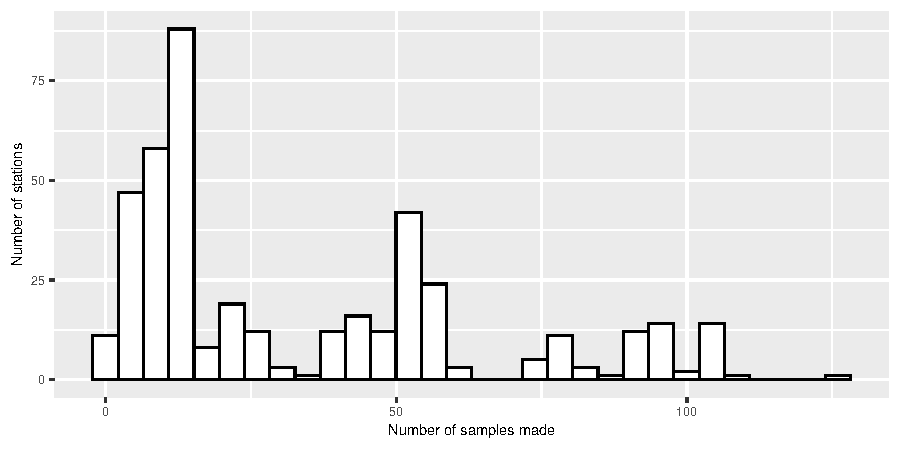
\includegraphics[]{figs/Chap5/hist_samp_sta.pdf}
  \caption{Distribution of the number of measurements per station.}
  \label{fig:histogram}
\end{figure}

The coarse representation $\overline{\mathcal{D}}$ of the monitoring data $\mathcal{D}$ is obtained by computing the maximum daily values across the available stations. This yields the time series illustrated in Figure \ref{time:serie}. The aggregated series contains $n =$ 2,150 values, among which 22.51\% are quantified. 

\begin{figure}[htbp]
  \centering
  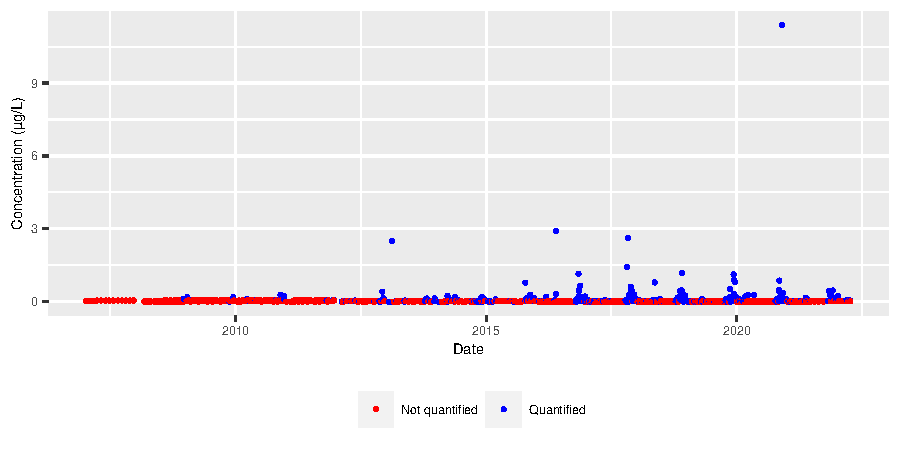
\includegraphics[]{figs/Chap5/Max_temp-1.pdf}
  \caption{Plot of daily maximum concentrations}
  \label{time:serie}
\end{figure}

One may note here that despite the aggregation process, the coarse series remains irregularly sampled, and that for about two thirds of the days included in the studied time span, no measurements were made. 

\subsection{Graphical representation of the station network}\label{subsection:graph:construct}

The stations network $G=(V,E)$ introduced in Section \ref{subsection:graph} is built using the hydrographic map of the Centre-Val de Loire region. Indeed, once the monitoring stations are geo-localized through their GPS coordinates, one still has to compute the edges between them, as well as the associated weights. 

For the data at hand, edges are determined using the river network. A database provided by the French National Institute of Geographic and Forest Information (IGN) \cite{IGN:BD:TOPO} contains a fine-grained description of rivers, encoded as sequences of hydrographic sections (or river sections). River sections are segments with constant geographic and hydrographic attributes. 

The procedure used for computing the edges in the stations network based on the river network may be summarised as follows:

%We now describe how we built graphs based on a given set of stations $V$, denoted $G=(V,E)$ :   

%the station graph  was
%The data collected did not allow to build it directly because the geolocalisation information of the stations and the hygrographic network come from two disctinctive sources. 

\begin{enumerate}
    \item One starts by building a river network $\mathcal{R}=(S,H)$, where the vertices $S$ are made of the connecting points between the river sections, and the edges $H$ contain all sections. Each edge is thus naturally weighted by the length (in meters) of the corresponding river section. 
    \item Each monitoring station $v_i$ in $V$ is assigned to the closest node $\tilde s_i$ in the river network $R$, by minimizing the geographical distance between the station $v_i$ and all connecting points
    \begin{equation*}
     \tilde s_i=\min_{s\in S} d(v_i, s).
    \end{equation*}
    \item Given two stations $v_i,v_j \in V$ and their associated connecting points $\tilde s_i,\tilde s_j \in S$, an edge will be generated between $v_i$ and $v_j$ if there exists at least one path between $\tilde s_i$ and $\tilde s_j$. Furthermore, the weight associated to an edge $(v_i,v_j)$ is equal to the length of the shortest path between $\tilde s_i$ and $\tilde s_j$.
\end{enumerate}

One may notice at this point that the above procedure may result into an unconnected graph, with several connected components. For illustration, Figure \ref{fig:comp} displays the graph of all stations that made at least one sample during the obsetvation period. It is not fully connected and exhibits 9 distinct connected components.  

\begin{figure}[htbp]
  \centering
  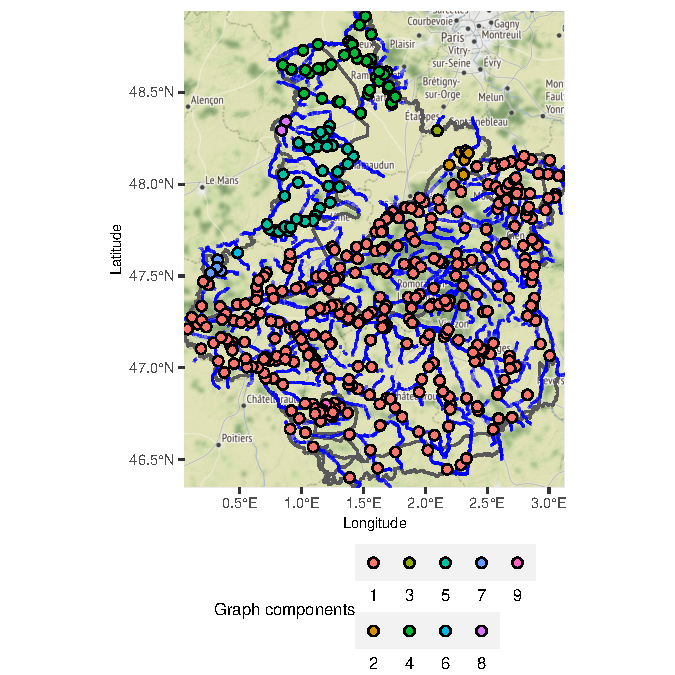
\includegraphics[]{figs/Chap5/Graph_comp-1.pdf}
  \caption{Map of the non connex components in the station graph.}
  \label{fig:comp}
\end{figure}

\section{Results}\label{section:results}

\subsection{Temporal segmentation}\label{sec:time_pattern}

First, the coarse-grained time series $\overline{\mathcal{D}}$ in Figure \ref{time:serie} is segmented using the change-point detection procedure described in Section \ref{chp:4:3}. We fitted a left censored Weibull distribution in the change-point model with parameters $(\lambda,\sigma)$. This was motivated by the observation of the data. We suppose $\sigma$ fixed in the time series and propose the heuristic \ref{chp:4:3} to estimate it. The results of its estimation are shown in Figure \ref{fig:sig}.

\begin{figure}[htbp]
  \centering
  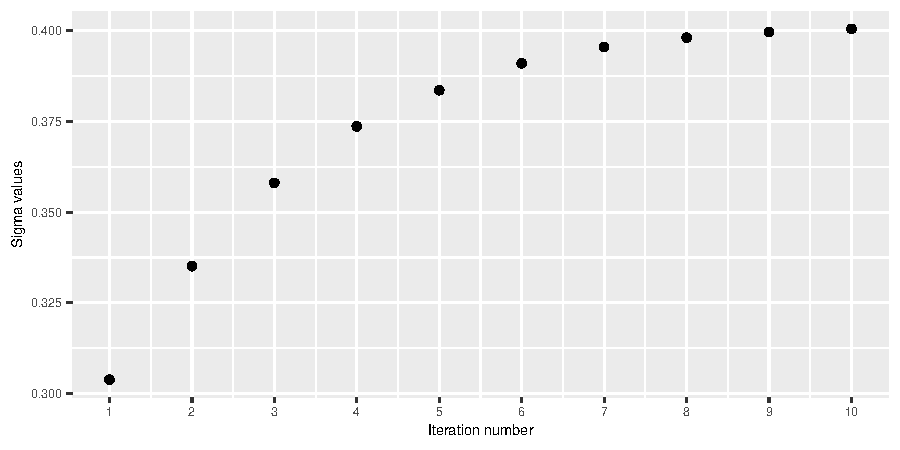
\includegraphics[]{figs/Chap5/Sigma_heu.pdf}
  \caption{Plot of successive $\widehat{\sigma}$ values. We stopped the to iterate when the $\lvert \widehat{\sigma}_{b-1} - \widehat{\sigma}_{b} \rvert \leq 10^{-3}$}
  \label{fig:sig}
\end{figure}

The penalty grid $[\frac{\ln n}{4},4\ln n]$ was chosen for the heuristic where $n$ is the number of daily maximum concentrations available, here $n = 2150$. This interval allowed to obtain various segmentation results with the number of change points varying from 1 to 30. With such kind of range in the results, it ensured a central position of the elbow in the plot of the cost of these segmentations against their respective number of change-points. The precision stopping criterion was set to $10^-3$.
From the application point of view, the assumption that $\sigma$ is a fixed parameter throughout the series $\overline{\mathcal{D}}$ corresponds to the hypothesis that the differences in usage and diffusion of the prosulfocarb among the different users is captured by the shape parameter, and should not vary much over time. On the contrary, the overall average usage of prosulfocarb varies, and this dependency is captured by changes in the rate parameter. Let us remark here that the estimated value of the shape parameter is $\hat \sigma_{MLE}=0.4$. This confirms the data has a heavier tail than an exponential distribution ($\sigma$=1), and that the assumption of using Weibull distributions for our data is appropriate. 

%Then, to detect temporal patterns the PELT algorithm was used with a minimal segment length of $50$ days. 

In the change-point detection procedure, the penalty value for the PELT algorithm was calibrated using a large range of values explored according to the CROPS algorithm. The range, inspired by the BIC criterion, was set to $[\frac{\log(n)}{5},5\log(n)]$. Note that when using the BIC penalty in change point detection, the penalty term written becomes : $\beta_n(K+1)|\mathcal{M}| = \frac{|\mathcal{M}|}{2}\log(n)(K+1) = \frac{1}{2}\log(n)(K+1)$ where $|\mathcal{M}|$ is the cardinal of the dimensions of the parameters $\bm\theta$ of $Q$ that are subject to changes across segments. Since $\bm\theta = (\lambda,\sigma)$ and the changes occur only on the $\lambda$ parameter, $|\mathcal{M}| = 1$. The range chosen allows to screen an interval of penalties containing the BIC penalty.

The penalty calibration procedure resulted in 15 different segmentations, with a number of change-points ranging from 1 to 30. The best segmentation is selected using the elbow method, as illustrated in Figure \ref{fig:elb_seg} in Appendix \ref{section:elb}. This amounts to a temporal segmentation with $\hat K=13$ change-points, illustrated in Figure \ref{fig:seg}. 
%Some similar procedures are found in \cite{lung2015homogeneity}. 
 
\begin{figure}[htbp]
  \centering
  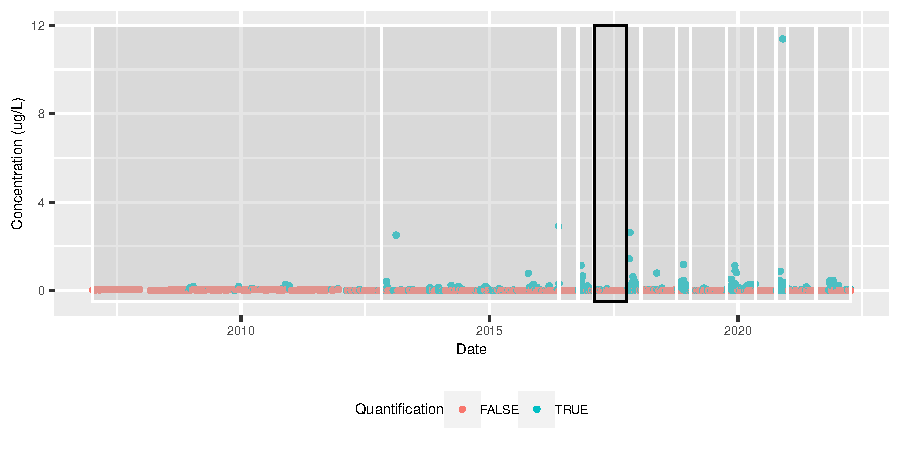
\includegraphics[]{figs/Chap5/Seg_opt.pdf}
  \caption{Best segmentation found by the change-point detection procedure with CROPS-based penalty tuning. The dates of the breaks are : October 20, 2012; May 25, 2016; October 13, 2016; February 7, 2017; October 5, 2017; January 19, 2018; October 5, 2018; January 18, 2019; October 11, 2019; May 6, 2020; October 7, 2020; December 20, 2020; July 27, 2021.The black rectangle corresponds to the selected temporal segment in section \ref{section:clust129}}\label{fig:seg}
\end{figure}

According to Figure \ref{fig:seg}, the usage of prosulfocarb in Centre-Val de Loire shows different patterns throughout time. Before 2016, most of the values are not quantified, and there are almost no change-points detected. Starting with 2016, two regimes of pesticide usage appear to emerge, and correspond respectively to the periods of intensive usage of prosulfocarb and to the off-peak periods. Indeed, the starting dates of the peak periods coincide with the season where the substance is spread, which is Autumn. The emergence of this two-regime pattern, alternating high concentration values during the peak periods and low concentration values during the off-peaks, is correlated with an important increase in the prosulfocarb sales as shown in Figure \ref{fig:sale} in Appendix \ref{section:sale}. 

\subsection{Spatial segmentation}\label{section:clust129}

The second step of the analysis consists in the spatial segmentation using the graph-based clustering on the monitoring stations network. This step is strictly independent from the temporal segmentation. 

During the whole observation period, 420 monitoring stations only produced at least one measure. The spatial clustering algorithm was applied with a number of potential clusters varying between 7 and 35. The minimum number of clusters is equal to the number of connected components in the graph composed of more than one station plus one cluster. There are 6 components with more than one station and we add a supplementary cluster at the initialisation of the clustering procedure. The optimal number of clusters was selected using the elbow method applied to the inertia curve. According to this criterion, illustrated in Figure  in Appendix \ref{section:elb}, the best solution is made of a 15-clusters configuration. The spatial segmentation is illustrated in Figure \ref{fig:clust}. The algorithm based on dynamic programming \ref{algo:dyn} was used to create the partition of the station graph.
%(the minimum number of clusters is equal to the number of connected components in the graph induced by the active stations)
To check the relevance of the homogeneity assumption formulated in section \ref{section:spaceclust}, let us focus on a specific temporal segment. An off-peak period, spanning between February 8, 2017 and October 4, 2017 was selected. This period was identified as a homogeneous temporal segment by the change-point detection procedure.  This period is highlighted by the black rectangle in Figure \ref{fig:seg}. We proceeded in two steps. First we pooled all samples made during that specific period of time. From all those samples, we can identified the active clusters during that period of time, there were 13 out of 15. Then, for all active clusters, we computed the within average empirical pairwise Wasserstein distance of the active stations of a cluster and observe that for 10 clusters out of 13, this indicator is less than 0.0015, whereas the global average pairwise Wasserstein distance for the 149 stations is 0.003. This suggests that the distance chosen for our station graph is indeed a good proxy of the homogeneity in the concentration space. Additional comments can be made when we look at the geography of the region. Some clusters are overlapping with hydro-ecoregions. Hydro-ecoregions are geographic entities in which hydrographic ecosystems share common characteristics. The criteria defining them combine properties of geology, terrain and climate \cite{wasson:hal-02580774}. The borders of those regions are drawn in grey in Figure . This ensures that the substances will have homogeneous dispersion properties on these clusters (see clusters 7). As expected the biggest component in Figure \ref{fig:comp} is the most segmented. Some clusters are easy to identify, for instance clusters 12 corresponds to the Indre river. Cluster 10 is identified as the most western part of the Loire and its tributaries mainly the Vienne and the Creuse rivers. Clusters 1,7,9 and 10 are a little bit harder to identify. If one look closely at the map of the region, there is a high presence of small channels all across this part of the region. 

\begin{figure}[htbp]
  \centering
  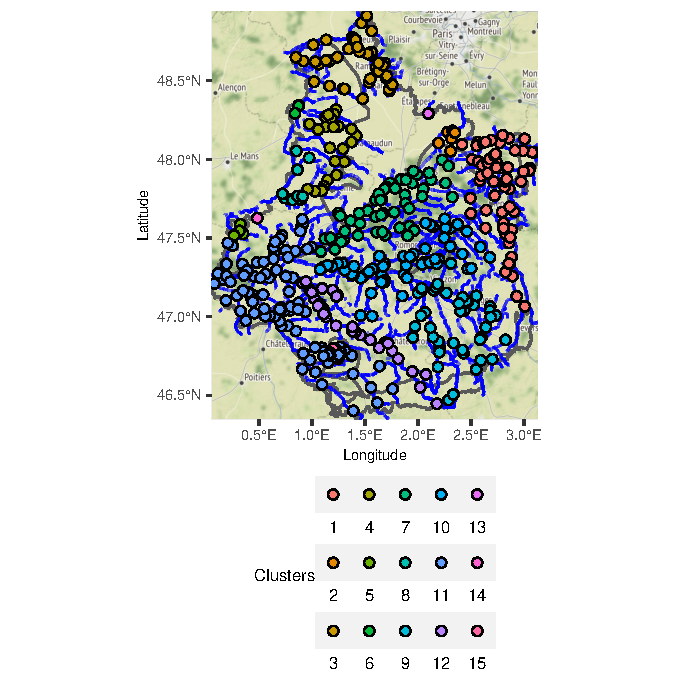
\includegraphics[]{figs/Chap5/Graph_clust.pdf}
  \caption{Map of geographical clusters.}
  \label{fig:clust}
\end{figure}

\subsection{Anomalous cluster identification}\label{subsection:anomalous}

We now focus on locating spatial patterns during time segments identified in section \ref{sec:time_pattern}. Peak periods in prosulfocarb use are less likely to produce rich spatial patterns since they correspond to a intensive overall use in the region. This why an off-peak period was investigated instead. In the rest of this case study, we selected the segment highlighted in black in figure \ref{fig:seg}. It is delimited by the dates February 8, 2017 and October 4, 2017. This introduces a context to the anomaly detection: a global non use of the substance. 

\begin{figure}[htbp]
  \centering
  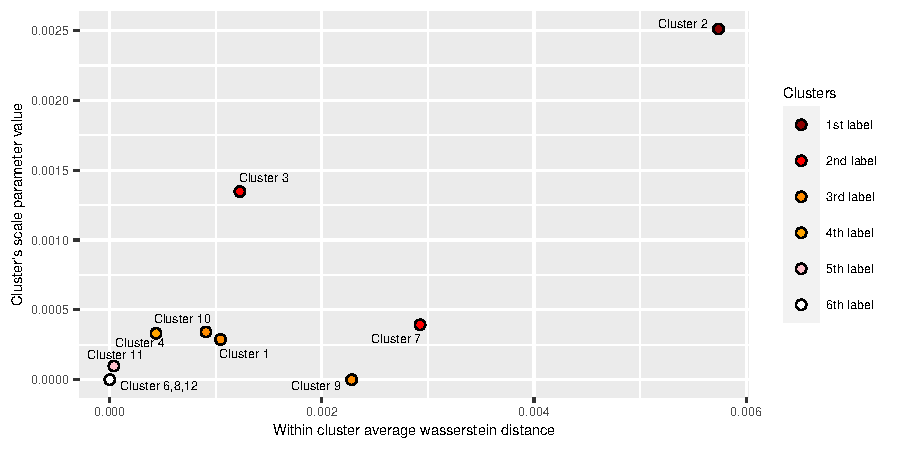
\includegraphics[]{figs/Chap5/Pareto_plot.pdf}
  \caption{Clusters pareto front.}
  \label{fig:pareto:plot}
\end{figure}

 %More precisely, high values of $\frac{1}{\lambda_k}$ are related to observed high values in the concentrations, while high values in $\bar{W}_k$ denote high heterogeneity in the stations distributions.
%summarise the homogeneity of the concentration distributions of its stations $v_j$ and the intensity of its concentration values respectively. 

Following the methodology proposed in \ref{section:anomaly}, the scaling parameter $\lambda_k$ of the aggregated data of each spatial cluster found in Section \ref{section:clust129} was estimated. The statistics $\bar{I}_k$ was set to $1/\hat{\lambda}_k$. The Pareto front involving the two descriptors $\bar{W}_k$ and $\bar{I}_k$ was computed. It led to the cluster ranking displayed in Figure \ref{fig:pareto:plot} using the \emph{rPref} package \cite{RJ-2016-054}. We recall that the selected time segment corresponds to a period of non-use of prosulfocarb. From this it can be deduced that finding quantified measurements of the substance during this period is an anomaly. Three clusters stood out with a Pareto front levels of 1 and 2. Among them we can find on Figure \ref{fig:pareto:plot}: 
\begin{itemize}
    \item \textbf{Cluster 2:} which is the most anomalous cluster. There is a bias coming from the number of samples made during that time period. Only 11 measures were reported. However, it is interesting to note that this cluster has a 27.27$\%$ rate of quantification which corresponds to 3 quantified measurements. The rate of quantification has a huge influence on the estimated scale parameter of the cluster. It is then logical to find this cluster dominating the other on this axis. This cluster didn't record the maximum concentration during the period but its highest quantification value is up to 0.031 $\mu$g/L which the third highest value recorded in the temporal segment. Combined with the high quantification rate, it implies that the mean within Wasserstein distance is elevated.  
    %a cluster which has recorded a very high concentration value but is composed of one station only, it corresponds to cluster 10 in Figure . Four measurements were made at that station among which one was quantified. It leads to a higher quantification rate than in the other clusters and high value of $1/\hat{\lambda}_k$.  
    %\ref{fig:graph}
    \item \textbf{Clusters 3 and 7:} which are Pareto level 2 clusters. Cluster 3 has a 6.09$\%$ quantification rate which higher than cluster 7 (4.48$\%$). This explains its higher position on the scale parameter estimate axis. Its maximum value is 0.039 $\mu$g/L which is smaller than the maximum in cluster 7 which is 0.087 $\mu$g/L. The difference in within Wasserstein distance is higher in cluster 7 because it has a station that made a very high quantification compare to other stations. the recorded 0.087 $\mu$g/L is actually the maximum of concentration of the whole temporal segment.
    %a cluster where one can find different profiles of stations. Some of them recorded high concentration values while the others did not provide any quantified measurement. It corresponds to cluster 4 in Figure . Nine stations compose this cluster. These stations performed 68 measurements among which five were quantified. The quantified measurements can be found in three different stations. 
    %\ref{fig:graph}
    %a cluster composed of 24 stations that recorded 99 samples. This cluster recorded the maximum level of concentration during the selected time segment. Only six measurements were quantified and they are distributed over three stations. It corresponds to cluster 5 in Figure . The low rate of quantification leads to a low value of $1/\hat{\lambda}_k$ but the heterogeneity between concentration profiles is higher given that the station that recorded the maximum is very abnormal.
    %\ref{fig:graph}
\end{itemize}

\begin{figure}[htbp]
  \centering
  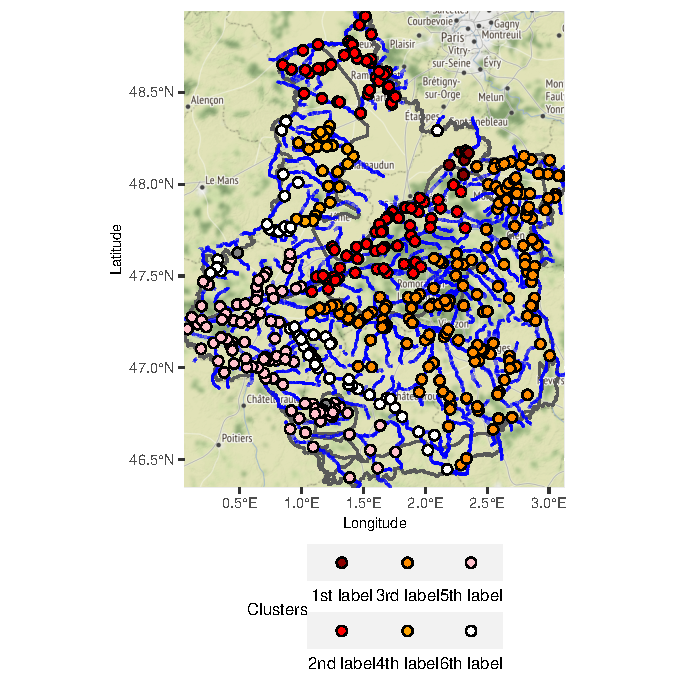
\includegraphics[]{figs/Chap5/Pareto_map.pdf}
  \caption{Mapped pareto front.}
  \label{fig:pareto:map}
\end{figure}

It is interesting to note that the Pareto front level is not uniformly distributed in the region. The three anomalous clusters are located in the north and east of the region. It could be related to the agricultural practices and land use. For the sake of the argument, we present in Appendix \ref{section:crops} the map of barley and wheat crops in Centre-Val de Loire. In future works, we shall investigate the spatial correlation between anomalous clusters and areas with high concentration of these crops. Figure  displays the Pareto front levels on the station map \ref{fig:pareto:map}.

\section{Chapter summary}

This Chapter presents the statistical analysis performed to monitore concentration data. The procedure is organized in three steps. The two first steps are independant and deals with the characteristics of concentration data presented in Chapter \ref{chp:2}. The first step is the temporal change-point detection method adapted for censored data developped in Chapter \ref{chp:4}. Homogeneous time segments are found in the aggregated time series of the daily maximum concentrations observed in the region of study. This step results in identifying the regimes of use of a substance in the region. The second step tackles the spatial heterogeneity. It is assumed that the environment in which the substance is diffusing explains most of the spatial heterogeneity in the concentration levels. Then, the second step consists in clustering the stations according to the environment structure. The environment structure constitutes a proxy that should capture geographical areas where the concentration levels should be homogenous. This clustering step is performed using Ward hierarchical clustering. The last step is to bring anomalous clusters out in the context of a temporal segment. This can be done using multi-criterion optimization. Each cluster found in the second step is characterized by two criterion that are calculated using all the concentration measures that were made by the stations cluster. The first criterion assess the presence of anomalous stations in the cluster, the second criterion assess the overall levels of concentration in the cluster. The Pareto front computed in the multi-criterion optimization allows to characterize the anomaly level of a cluster.  

All this procedure is illustrated on the prosulfocarb concentration in the Centre-Val de Loire region. The most important result is that Pareto front levels are not distributed uniformly on the region territory. This allows to identify "epicentre" of substance use in the region. This Chapter only presents the results for one temporal segment. Chapter \ref{chp:6} presents an interactive tool that allows such task. This constitutes the monitoring tool that ally statistical inference with visualization techniques that was mentionned in Chapter \ref{chp:2}. 
 